\documentclass[11pt]{article}
\usepackage{graphicx}
\DeclareGraphicsRule{.tif}{png}{.png}{`convert #1 `dirname #1`/`basename #1 .tif`.png}

\textwidth = 6.5 in
\textheight = 9 in
\oddsidemargin = 0.0 in
\evensidemargin = 0.0 in
\topmargin = 0.0 in
\headheight = 0.0 in
\headsep = 0.0 in
\parskip = 0.2in
\parindent = 0.0in
\usepackage{paralist} %compactenum

%\newtheorem{theorem}{Theorem}
%\newtheorem{corollary}[theorem]{Corollary}
%\newtheorem{definition}{Definition}
\usepackage{tipa}
\usepackage{amsfonts}
\usepackage[mathscr]{eucal}

% Use the natbib package for the bibliography
\usepackage[round]{natbib}
\bibliographystyle{apalike}
\newcommand{\exampleMacro}[1]{\mu_{#1}}

\title{Brief Article}
\author{The Author}

\usepackage{url}
\usepackage{hyperref}
\hypersetup{backref,  pdfpagemode=FullScreen,  linkcolor=blue, citecolor=red, colorlinks=true, hyperindex=true}

\begin{document}
You have studied bill width in a population of finches for many years. You record your data in units of the standard deviation of the population, and you subtract the average bill width from all of your previous studies of the population.
Thus, if the bill widths are not changing year-to-year and they are distributed according the Normal distribution (as many quantitative traits are), then your data should be described by $\mathcal{N}(0,1)$.

{\it Problem}: 
Consider the following data set collected from 5 randomly sampled birds following from this population, but following a year of drought:
\begin{center}
\begin{tabular}{c|c}
Indiv. & standardized bill width \\
\hline
1 & 0.01009121 \\
2 & 3.63415088 \\
3 &-1.40851589 \\
4 & 3.70573177 \\
5 &-0.94145782
\end{tabular}
\end{center}
Oddly enough it appears that you have enough money to measure bill widths using an SEM (based on the ridiculous number of digits in your measurments), but you can only catch 5 finches.\\
{\bf Can you conclude that the mean bill width in the population has changed?}

{\it Solution}: If you talk to someone without any statistical training (and then translate their answer into stats jargon), they will say that we should answer this by:
\begin{compactenum}
	\item estimating the mean based on the data (estimate $\hat{\mu}$), and then
	\item see if $\hat{\mu} = 0$.
\end{compactenum}
But this clearly ignores the fact that our estimate will be affected by sampling error (so we'll conclude there has been a change in the mean any time we do the test).

If you ask someone trained in  Neyman-Pearson style of hypothesis testing they'll say that we should:
\begin{compactenum}
	\item state the {\em null hypothesis} ($H_0: \mu = 0$, in this case);
	\item stat the {\em alternative hypotheses} ($H_A: \mu\neq0$ in this case);
	\item choose a {\em test statistic};
	\item choose your {\em Type I error rate} (usually denoted $\alpha$) to be what you consider to be an acceptable probability of rejecting a null hypothesis when it is true.
	\item determine the {\em null distribution} of the test statistic - the frequency distribution of the values of the statistic that we would see if the null hypothesis were true.
	\item from the null distribution of the test statistic, the Type I error rate, and the knowledge of what values of the test statistic are more compatible with the alternative hypothesis than the null, you can determine the {\em critical value} of your test statistic.
	\item If the value of the test statistic calculated on the real data is more extreme than the critical value, then you reject the null.
\end{compactenum}
This is a general procedure. 
Which test statistic you should use is not always obvious.

The \href{http://en.wikipedia.org/wiki/Neyman%E2%80%93Pearson_lemma}{Neyman-Pearson lemma}
states that we should use the likelihood ratio test-statistic if we are testing two distinct points (e.g. if $H_0: \mu=0$ and $H_A: \mu=1$ for example).
The lemma actually states that the likelihood ratio test-statistic is the most powerful (e.g. gives us the most power to reject the null when it is false) that is ``honest'' in the sense of guaranteeing it reported Type I error rate.

In our case, we do not have a distinct hypothesis (``point hypothesis'') as an alternative.  
But we can still use the likelihood ratio as our test statistic, but we have to have a pair of points to use when calculating the test statistic.
We can use the MLE when calculating the likelihood that is in the denominator in the ratio, and we can use the null hypothesis' value of $\mu$ when calculating the numerator.
We also take the log of the ratio and multiply it by -2 (so that the properties that we proved in problem \#3 of homework \#2 hold): 
$$ -2\ln\Lambda =  2 \ln[L(\hat{\mu})] - 2\ln[L(\mu_0)].$$



As you may recall from the second homework:
\begin{eqnarray*}
	L(\mu) & = &\Pr(X|\mu) \\
		& = & \prod_{i=1}^{n}\Pr(x_i|\mu)\\
		& = & \prod_{i=1}^{n}\frac{1}{\sqrt{2\pi\sigma^2}}e^{-\frac{(x_i-\mu)^2}{2\sigma^2}} \\
\end{eqnarray*}
If we assume that $\sigma=1$ then we also showed that:
\begin{eqnarray*}
	\ln [L(\mu)] & = & n\ln\left(\frac{1}{\sqrt{2\pi}}\right) - \left(\sum_{i=1}^{n}\frac{x_i^2}{2}\right) + n\bar{x}\mu - \frac{n\mu^2}{2} \\
	\hat{\mu} & = & \bar{x} = \frac{\sum_i^n x}{n}
\end{eqnarray*}
For the data set shown above $\hat{\mu} = \bar{x} = 1$, and our null dictates that $\mu_0 = 0$.  We can also calculate that: $0.5*\sum_{i=1}^{5}x_i^2 = 14.90493$ and $5\ln\left(\frac{1}{\sqrt{2\pi}}\right) = 4.59469$ for our data set.
This lets us conveniently express the log-likelihood as:
\begin{eqnarray*}
	\ln [L(\mu)] & = & 19.49962 + \left(\sum_{i=1}^{5}x_i\mu\right) - \frac{5\mu^2}{2} \\
	\ln [L(\mu)] & = & 19.49962 + 5\mu - \frac{5\mu^2}{2} \\
		& = & 19.49962 + \mu - 2.5\mu^2 \\
	\hat{\mu} & = & \bar{x} = \frac{\sum_i^n x}{n}\\
	\ln [L(\mu_0)] & = & -19.4996 \\
	\ln [L(\hat{\mu})] & = & -16.9996 \\
	-2\ln\Lambda & = & 5
\end{eqnarray*}
You will recall (from lecture and the homework) that know the null distribution of the LR test statistic in cases like this one (in which the MLE is not at a boundary, we are test a general model against a more specific ``nested'' form of the model, and the likelihood curve looks like a normal).
The null distribution is simply $\chi_k^2$ where the degrees of freedom, $k$, is simply to the number of parameters that are free to vary in the more complex (less constrained) model ($H_A$) but are fixed in the more simple model ($H_0$).

The critical value for $\chi_1^2 = 3.84$.  Our observed test statistic is greater than this, so we can reject the null.

It may be helpful to plot the $\ln[L(\mu)]$ for different values of $\mu$. In this case the plot is simply a parabola with the maximum point at $\mu=1$:\\
\begin{picture}(100,180)(-0,-160)
	\put(0,5){\makebox(-0,-150)[l]{\includegraphics[scale=0.6]{logLRAroundMLEforSIs1.pdf}}}
\end{picture}\\
the horizontal line is at -18.9196, which is 1.92 below the maximum likelihood score.  1.92 is chosen because twice this value corresponds to 3.84 (our critical value).
If we were to test a null hypothesis that $\mu$ takes a particular value, and the log-likelihood is below this threshold then we could reject the null\footnote{We are supposed to construct our null befor the test - this is just a thought experiment.}.
This means that we could construct a 95\% confidence interval based on where the log-likelihood intersects with the threshold score.
In this case, the confidence interval would be $0.123644 \leq \mu \leq 1.87636$, which does not include our null point ($\mu=0$).

Let us pause a note that we just did a hypothesis test, but we could also view this as an exercise in model selection.
We contrasted a zero-parameter model $\mathcal{N}(0,1)$ to a one-parameter model, $\mathcal{N}(\mu,1)$, and asked whether we could reject the simpler model.-
This is the  likelihood-ratio test approach to model testing.
Essentially the attitude is: only use a more complex model if the data warrants it, and we can assess this by performing a hypothesis test.
If we reject the simpler model, then we feel justified in using the more complex model.

OK, so it appears that we have evidence that the mean bill width has changed\footnote{The use of the LR test statistic gives us confidence that we have used the most powerful test, but the fact that the LR is monotonic function of the distance between $\bar{x}$ and the hypothesized mean ($\mu$) guarantees that we could have conducted an equally powerful test using $\bar{x}$ as our test statistic.  So the typical Z-test that may have occurred to you is just as good as the LR test in this case.}.
But if we have evidence that the distribution of bill widths has changed, can we really trust the applicability of the standard deviation from previous studies?

It would be safer to admit that we don't know the correct value of $\sigma$.
We can do this, but we will have a likelihood function with multiple parameters:

\begin{eqnarray*}
	L(\mu,\sigma) & = & \prod_{i=1}^{n}\frac{1}{\sqrt{2\pi\sigma^2}}e^{-\frac{(x_i-\mu)^2}{2\sigma^2}} \\
	\ln [L(\mu,\sigma)] & = & n\ln\left(\frac{1}{\sigma\sqrt{2\pi}}\right) - \left(\sum_{i=1}^{n}\frac{x_i^2}{2\sigma^2}\right) + \frac{n\bar{x}\mu}{\sigma^2} - \frac{n\mu^2}{2\sigma^2}\\
		& = & -n\ln\left(\sigma\sqrt{2\pi}\right) - \frac{1}{2\sigma^2}\left[\left(\sum_{i=1}^{n}\frac{x_i^2}{2}\right) + n\bar{x}\mu - \frac{n\mu^2}{2}\right]
\end{eqnarray*}
This likelihood function is defined over a 2-D space of parameter values.  Specifically, $-\infty<\mu<\infty$ and $0\leq\sigma<\infty$.
We are interested in finding the maximum point. 
It could occur at a boundary of parameters (although in this case the only boundary is $\sigma=0$ and clearly the data are not consistent with no variance in bill width, so that should not be a maximum likelihood point).
For an ``internal'' (non-boundary) point when we have a continuous and differentiable log-likelihood we are looking for a point at which the slope of the log-likelihood with respect to each of the parameters is zero (and the second derivatives are negative).
\begin{eqnarray*}
	\frac{\partial\ln [L(\mu,\sigma)]}{\partial \mu} & = & \frac{n\bar{x}}\sigma - \frac{n\mu}{\sigma} \\
	\frac{n\bar{x}}\sigma - \frac{n\hat{\mu}}{\sigma} & = & 0\\ 
	\hat{\mu} & = & \bar{x}
\end{eqnarray*}
In general, the first derivative with respect to one parameter will be a function of the other parameters. 
In this special case, the $\sigma$ in the first derivative wrt $\mu$ cancel out.
This makes some sense: $\mu$ is the ``center'' of the distribution. 
While changing the variance of the model will affect how well it fits the data, it won't make us change where we think the center of the distribution is. 
So the MLE of $\mu$ is simply $\bar{x}$ regardless of the value of $\sigma$.
When we want to estimate $\hat{\sigma}$ we see that this is not the case:
\begin{eqnarray*}
	\frac{\partial\ln [L(\mu,\sigma)]}{\partial \sigma} & = & \frac{-n\sqrt{2\pi}}{\sigma\sqrt{2\pi}} + \frac{\sum_{i=1}^n\left(x_i-\mu\right)^3}{\sigma^2} \\
	 & = & \frac{-n}{\sigma} + \frac{\sum_{i=1}^n\left(x_i-\mu\right)^2}{\sigma^3} \\
	 & = & \frac{1}{\sigma}\left[ -n+ \frac{\sum_{i=1}^n\left(x_i-\mu\right)^2}{\sigma^3}\right] \\
	 \frac{1}{\hat{\sigma}}\left[ -n+ \frac{\sum_{i=1}^n\left(x_i-\mu\right)^2}{\hat{\sigma}^2}\right] & = & 0
\end{eqnarray*}
The derivative equals zero if $1/\hat{\sigma}$ becomes zero\footnote{Because $\sigma<\infty$ this point is never reached.  But it does make sense that as you increase the variance to huge values, the likelihood stops changing much.} or:
\begin{eqnarray*}
	n & = &  \frac{\sum_{i=1}^n\left(x_i-\mu\right)^2}{\hat{\sigma}^2} \\
	\hat{\sigma} & = & \sqrt{\frac{\sum_{i=1}^n\left(x_i-\mu\right)^2}{n}}
\end{eqnarray*}
This should look familiar -- it is the ``population variance'' estimator.\footnote{We are used to seeing the sample variance, which looks similar but has $n-1$ in the denominator. The sample variance is an unbiased estimator, while the MLE is biased in this case (although the bias becomes negligible as $n$ increases).}
Note that the estimate of the standard deviation {\em does} depend on the value of $\mu$. If we are contemplating a value of $\mu$ that is close to $\bar{x}$, then the deviations between the observations and $\mu$ will be as small as we can make them; thus small variances will be inferred.  

If we are considering a value of $\mu$ that is very far from $\bar{x}$, then the data will appear to be far from the population mean. The best way to explain this data is to infer a large value for $\sigma$.

The maximum likelihood point, will jointly maximize both derivatives:
$$ (\hat\mu,\hat\sigma) = (\bar{x}, \sqrt{\frac{\sum_{i=1}^n\left(x_i-\bar{x}\right)^2}{n}})$$
(note that we substitute $\bar{x}$ in for $\mu$ because we want $\hat\sigma$ calculated at $\hat\mu$).

For the data set that we are contemplating:
\begin{eqnarray*}
	 (\hat\mu,\hat\sigma) & = & (1, 2.22755) \\
	 \ln\left[L(\mu=1, \sigma=2.22755)\right] & = & -11.0992
\end{eqnarray*}
Note that the standard deviation based on the data that we collected is much larger than 1, so our previous assumption of $\mathcal{N}(\mu,1)$ may indeed be suspect.

How can we test if we can reject $H_0: \mu=0$?  It may be tempting to simply use the value of $\hat\sigma$ that maximizes the likelihood:
$$	 \ln\left[L(\mu=0,\sigma=2.22755)\right]  = -11.603 $$
but this is not appropriate. Recall that $\hat\sigma$ is a function of the data and of $\mu$, so if we want to reject $\mu=0$ we should use the standard deviation that fits best we with this value of $\mu$:
\begin{eqnarray*}
	 \hat\sigma_{\mu_0} & = & 2.44171 \\
	 \ln\left[L(\mu=0,\sigma=2.44171)\right] & = & -11.5582
\end{eqnarray*}
Note that the estimate of the standard deviation has increased. Now our LR test statistic is much smaller:
\begin{eqnarray*}
	 -2\left(\ln\left[L(\mu_0,\hat\sigma_{\mu_0})\right] - \ln\left[L(\hat\mu,\hat\sigma)\right]\right) & = & -2(-11.5582 + 11.0992) \\
	 & = &  0.918
\end{eqnarray*}
This is not significant. 
Thus we cannot reject $\mu_0$ if we admit the the standard deviation may have changed.

The trace plot below shows the log-likelihood as a function of $\sigma$ for $\mu=-1$ (black), $\mu=0$ (blue), and $\mu=1$ (red).
Note that the MLE of $\sigma$ gets larger as the $\mu$ moves away from $\bar{x}$ (which is 1 for these data), but in all cases the log-likelihood is much lower if we consider $\sigma=0$. \\
\begin{picture}(200,180)(-0,-160)
	\put(0,5){\makebox(-0,-150)[l]{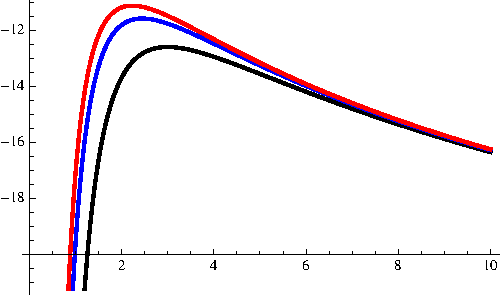
\includegraphics[scale=.9]{profileOfStdDevForDiffMu.pdf}}}
\end{picture}\\

The figure below shows three different tests of $H_0: \mu=0$. In blue we has a LR ratio test that (incorrectly) fixes $\sigma=1$ (the horizontal line is the threshold for rejection). Note that the confidence interval is narrow, and we seem to have a lot of power to reject different values of $\mu$.
Statistical power is good; but, in this case, we are getting the power by making an unjustified assumption (that $\sigma$ has not changed).
LR tests that admit we do not know $\sigma$ are shown in red (for cases in which we estimate $\hat\sigma$ for each different $\mu$ value that we consider), and green (for cases in which we estimate $(\hat\mu,\hat\sigma)$ and then treat $\hat\sigma$ as if it were applicable to all values of $\mu$).\\
\begin{picture}(200,180)(-0,-160)
	\put(0,5){\makebox(-0,-150)[l]{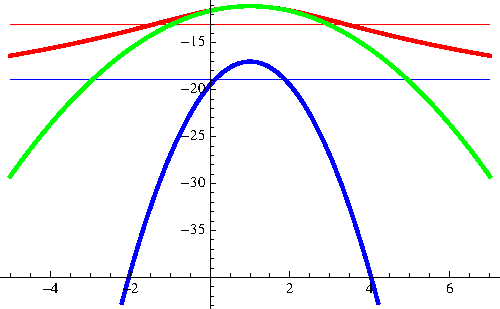
\includegraphics[scale=.9]{SigTestsOfMu.pdf}}}
\end{picture}\\
The curve in red is the correct way to perform the test. In creating this curve we consider a wide range of $\sigma$ values, and we essentially admit that we don't know what the truth is.
In the green curve, the $\hat\mu$ point ``gets'' to have its preferred $\sigma$, but all other points are evaluated at a standard deviation ($\hat\sigma_{\hat\mu}$) that is not as compatible as possible.  Thus, we get a narrow confidence interval, but once again it is unjustified power. 

If we were to do a simulation study only the method shown in red would have the correct Type I error rate (the others would reject too often).

We could also do a hypothesis test of $\sigma=1$. In this case we would reject.

What about if we wanted to test the hypothesis that the distribution is still $\mathcal{N}(0,1)$? We can compare the $\ln\left[L(\mu=0,\sigma=1)\right]$ to $\ln\left[L(\hat\mu,\hat\sigma)\right]$, as you might expect.  
Interestingly, we should compare the test statistic to $\chi_2^2$ rather than $\chi_1^2$, because there would be two parameters that are constrained in the null but not are estimated in our ``free-est'' model.
The critical value would be 5.99 (blue and pale areas below) rather than 3.84 (pale area below):\\
\begin{picture}(200,180)(-0,-160)
	\put(0,5){\makebox(-0,-150)[l]{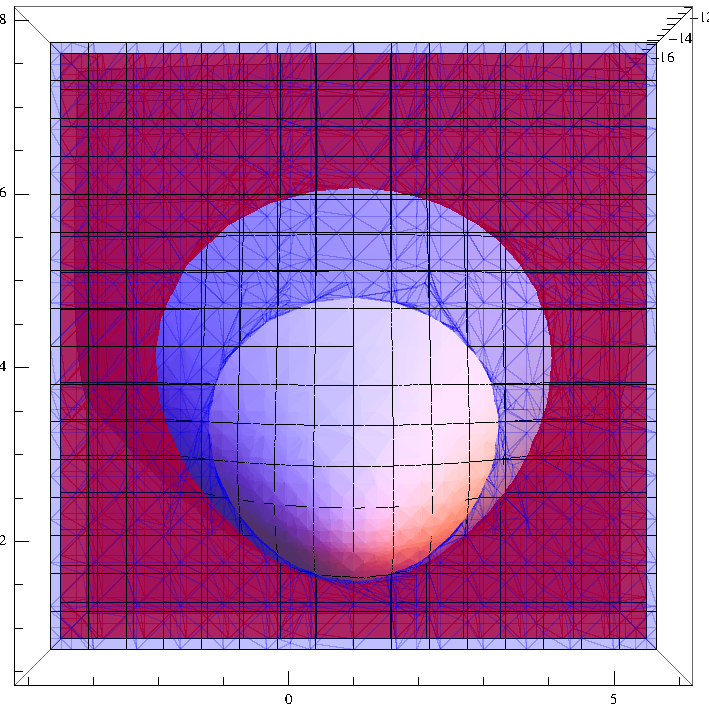
\includegraphics[scale=.5]{TwoParamNormalFromTop.pdf}}}
\end{picture}\\


It is possible that one group of researchers investigating $H_0: \mu=0$ would reject the null, another group testing $H_0: \sigma=1$ would reject their null, but a third group investigating $H_0: \mu=0, \sigma=1$ would {\em not} reject!
Thus it is important to frame your hypothesis carefully if you need to maximize power.
\footnote{In the numerical example given above, any of these three nulls would be rejected.}

We have a higher threshold of LR test statistic to surpass when we are comparing models that differ my more dimensions.  
You can think of each parameter leading to a certain amount of sampling error. 
Imagine that the null is true. Sampling error in a likelihood context means that $\hat\theta\neq\theta$, and by definition of an MLE we know that $\ln[L(\hat\theta)]\geq\ln[L(\theta)]$.
Thus each new parameter boosts the log-likelihood score of the point that corresponds to the MLE above the log-likelihood evaluated at the true parameter values.

You proved in the homework that the distribution of the difference in log-likelihoods between the true point and the MLE was the square of a Z-score. When you sum up the effect of $k$ parameters, it is like summing the squares of $k$ variables drawn from $\mathcal{N}(0,1)$.  
This is the $\chi_k^2$ distribution.

\subsection*{Summary of example}
\begin{itemize}
	\item We can use the LR Test for model choice and hypothesis testing - indeed it leads to the most powerful hypothesis tests.
	\item If we do not know the value of a parameter that occurs in the likelihood equation, we can estimate it.
	\item Even if we don't care about the parameter (e.g. $\sigma$ in our original question); its value can affect our hypothesis tests. Such parameters are typically referred to as ``nuisance parameters''
	\item Adding more parameters can increase realism (or at least more accurately reflect our ignorance), but the cost is less certainty in our estimates of the parameters that we care about (compare the red and green lines in the profile of $\ln L(\mu)$, and pretend that the green line represents a case in which we {\em knew} the correct value of the standard deviation).  In other problems, adding a nuisance parameter will actually increase $\mathbb{E}(|\hat\theta - \theta|)$
	\item When the likelihood around the MLE looks ``normalish'' (not at a boundary and not a weird likelihood function), then the the $\chi_k^2$ distribution does a nice job of describing the null distribution of the LRT statistic.  We'll talk about what to do when this is not the case later (e.g. parametric bootstrapping).
\end{itemize}

\section*{Alternative forms of model selection}
The following methods do not assume that models are nested:
\subsection*{Akaike Information Criterion}
	$$AIC(M|X) = 2k - 2 \ln L(\hat\theta | X, M)$$
You want to minimize this score (find the model $M$ that has the lowest AIC score for a dataset $X$)

Formulated based on information theory and measure how much information is lost when we use model $M$ to predict new data.
It is a bit unclear what conditions are required to make the AIC the appropriate choice 
More formally, the Kullback-Leibler distance is used to assess the discrepancy between the ``true'' and each model; You can think of the $2k$ term as a penalty for overfitting the data.

You can rank models by AIC and use the AIC scores as weights in multi-model inference.

Bayesians argue that the AIC ignores uncertainty in the nuisance parameters and thus tends to prefer models that have too many parameters.

\subsection*{Bayes Factors}
$B_{01}$ is the Bayes factor in favor of model 0 over model 1:
$$B_{01} = \frac{\Pr(X|M_0)}{\Pr(X|M_1)}$$
Note that this is just a likelihood ratio, but it is not the likelihood evaluated at it maximum, rather it is:
\begin{equation}
	\Pr(X|M_0) = \int \Pr(X|\theta_0)\Pr(\theta_0) d\theta_0) \label{margLike}
\end{equation}
where $\theta_0$ is the set of parameters in model 0.

Schwartz showed that this marginal likelihood (for the purpose of approximating Bayes factors) can be approximated by assigning a score to each model:
	$$BIC(M|X) = 2k\ln(n) - 2 \ln L(\hat\theta | X, M)$$

Better approximations of the Bayes factor are available, but they are usually much more expensive.
\subsection{Approximating marginal likelihoods using Laplace's method}
For example, we can use Laplace's method to approximate the integral in Eqn (\ref{margLike}); this method is based on approximating a function using a 
\href{http://en.wikipedia.org/wiki/Taylor%27s_theorem}{Taylor's  series}
 for approximating the value of a function at point $x$ given its value and derivatives at a nearby point, $x_0$:
\begin{eqnarray*}\nonumber
	g(x) & \approx &g(x_0) + \frac{1}{1!}\left(\frac{d g(x_0)}{d x}\right)(x-x_0) + \frac{1}{2!}\left(\frac{d^2 g(x_0)}{d x^2}\right)(x-x_0)^2 + \ldots + \frac{1}{n!}\left(\frac{d^n g(x_0)}{d x^n}\right)(x-x_0)^n 
\end{eqnarray*}
In particular, if we just use the first two derivatives in our approximation then:
\begin{eqnarray*}\nonumber
	g(x) & \approx &g(x_0) + \left(\frac{d g(x_0)}{d x}\right)(x-x_0) + \frac{1}{2}\left(\frac{d^2 g(x_0)}{d x^2}\right)(x-x_0)^2
\end{eqnarray*}
And if we are evaluating a likelihood function at its maximum point, then the first derivative should be 0, so:
\begin{eqnarray*}\nonumber
	L(\theta) & \approx &L(\hat\theta) +  \frac{1}{2}\left(\frac{d^2 L(\hat\theta)}{d \theta^2}\right)(\theta-\hat\theta)^2
\end{eqnarray*}

Laplace's method notes that for some large constant $M$, and a function evaluated at its maximum, $\hat\theta$:
\begin{eqnarray*}\nonumber
	g(\theta) & \approx & g(\hat\theta) -  \frac{1}{2}\left|\frac{d^2 g(\hat\theta)}{d \theta^2}\right|(\theta-\hat\theta)^2 \\
	e^{Mg(\theta)} & \approx & e^{Mg(\hat\theta) -  M\frac{1}{2}\left|\frac{d^2 g(\hat\theta)}{d \theta^2}\right|(\theta-\hat\theta)^2} \\
	               & = & e^{Mg(\hat\theta)}  e^{-M\frac{1}{2}\left|\frac{d^2 g(\hat\theta)}{d \theta^2}\right|(\theta-\hat\theta)^2} \\
	\int_a^b e^{Mg(\theta)} d\theta & \approx &  e^{Mg(\hat\theta)}   \int_a^b e^{\frac{-M\left|\frac{d^2 g(\hat\theta)}{d \theta^2}\right|(\theta-\hat\theta)^2}{2}}d\theta \\
	& \approx &  e^{Mg(\hat\theta)}   \sqrt{\frac{2\pi}{M\left|\frac{d^2 g(\hat\theta)}{d \theta^2}\right|}}
\end{eqnarray*}

So if we are interested in the integral of the likelihood, we can take the log-posterior density as our function $g(\theta)$:
\begin{eqnarray*}\nonumber
	\int \Pr(X|\theta)\Pr(\theta) d\theta & = & \int e^{\ln\left[\Pr(X|\theta)\Pr(\theta)\right]}d\theta\\
	& \approx & \sqrt{\frac{2\pi}{\left|\frac{d^2 \ln\left[\Pr(X|\tilde\theta)\Pr(\tilde\theta)\right]}{d \theta^2}\right|}}e^{\ln\left[\Pr(X|\tilde\theta)\Pr(\tilde\theta)\right]}\\
	& \approx & \left({\frac{2\pi}{\left|\frac{d^2 \ln\left[\Pr(X|\tilde\theta)\Pr(\tilde\theta)\right]}{d \theta^2}\right|}}\right)^{1/2}\left[\Pr(X|\tilde\theta)\Pr(\tilde\theta)\right]
\end{eqnarray*}
where $\tilde\theta$ denotes the point of maximum posterior probability density.
In the more general case of a $k$-dimensional model:
\begin{eqnarray*}
	\int \Pr(X|\theta)\Pr(\theta) d\theta & \approx & \left({2\pi}{\left|H(\tilde\theta)\right|^{-1}}\right)^{k/2}\left[\Pr(X|\tilde\theta)\Pr(\tilde\theta)\right]
\end{eqnarray*}
Where $H(\tilde\theta)$ is the Hessian matrix of second derivatives around the point of maximum posterior probability density.

You can also evaluate this around the MLE, $\hat\theta$, if the MAP is hard to find (or the prior information is very vague).

See \cite{KassR1995} for more details (that reference served as the basis for the previous section on Bayes Factors).
\bibliography{phylo}
\end{document}  
